
\newcommand{\etas}{\ensuremath{\eta_{\mathrm{s}}}}


\chapter{Background and Introduction}
Aerodynamic shape optimization of airship envelopes generally involves obtaining the shape having lowest volumetric drag coefficient ($C_{DV}$). Low drag shapes are preferred in airships because the power required for flight is directly proportional to the value of $C_{DV}$. Most existing studies related to shape optimization of airship envelopes assume them to be axi-symmetric bodies of revolution.

However, unconventional non axi-symmetric shape can provide many advantages over conventional axi-symmetric shapes. As can be seen in Fig. \ref{Stratellite}, they can have flatter upper surface, which is advantageous for capturing more solar irradiance in the case of stratospheric airships with solar panels on the top.
\begin{figure}[H]
	\centering
	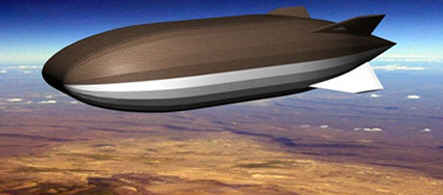
\includegraphics{intro/Stratellite.jpg}
	\caption{Airship with non-axisymmetric envelope [\citenum{stratellite}]}
	\label{Stratellite} %      only if needed 
\end{figure}

 Existing literature has good amount of work done on CFD analysis of axisymmetric shapes but not on non-axisymmetric shapes. The reason is obvious, 2D analysis can easily be done for axisymmetric shapes. But to analyze non-axisymmetric shapes, we need to perform 3D CFD analysis. It demands more computational power which might not be available for many researchers. An open source CFD software called OpenFOAM\textsuperscript{\textregistered} (Open source Field Operation And Manipulation) has been used in our present study to perform CFD analysis. OpenFOAM\textsuperscript{\textregistered} comes with an inbuilt meshing (\textit{Block mesh} and \textit{Snappy Hex Mesh}) and post-processing (\textit{Paraview}) utilities, both of which are known for their unique and advanced method of problem solving capabilities. \\

\section{Work done in the present study}
This study is divided into two parts. In the first part, OpenFOAM\textsuperscript{\textregistered} software is validated using existing CFD results available in the literature for four standard shapes. A framework for carrying out multi-disciplinary shape  optimization has been laid out. The framework is then implemented in second part and arrived at an optimal shape with respect to user requirements.
\section{Report layout}
\label{layout}

After providing a brief introduction to shape optimization outlining the aims and objectives of this study, Chapter \ref{literature} gives the detailed literature survey of various fields required for multi-disciplinary shape optimization. Chapter \ref{openfoam} gives a brief introduction about OpenFOAM and demonstrates the power and advantages of using OpenFOAM\textsuperscript{\textregistered}.
Mesh generation using \textit{SnappyHexMesh} is discussed in Section \ref{mesh}. Section \ref{results} validates the OpenFOAM\textsuperscript{\textregistered} software with four axisymmetric standard shapes available in literature. Chapter \ref{geometry}  explains the modified Gertler parameter technique used for the parameterization of geometry.

Chapter \ref{optimization} gives a brief overview of need for the surrogate model in the optimization routine and explains the concept of surrogate model, design of experiments and formulation of different surrogate models. Section \ref{test function} explains the SBDO technique using Himmelblau test function. It also validates the Genetic algorithm code by Xavier [\citenum{Xavier}] which is used in subsequent chapters.

Chapter \ref{Surrogate model for CFD} gives the design space and design of experiment study parameters which will be used while building surrogate model in Section \ref{Training data CFD}. Running the actual CFD simulations for building surrogate model of CFD is done in Section \ref{Training data CFD}. Chapter \ref{Hoop stress} explains the concept of von-Mises stress and also gives the methodology to calculate it as given by Alam [\citenum{alam2017thesis}]. The results obtained while performing multi-disciplinary optimization of aerodynamic drag combined with von-Mises stress are presented in Chapter \ref{Final results}.

\begin{figure}[H]
	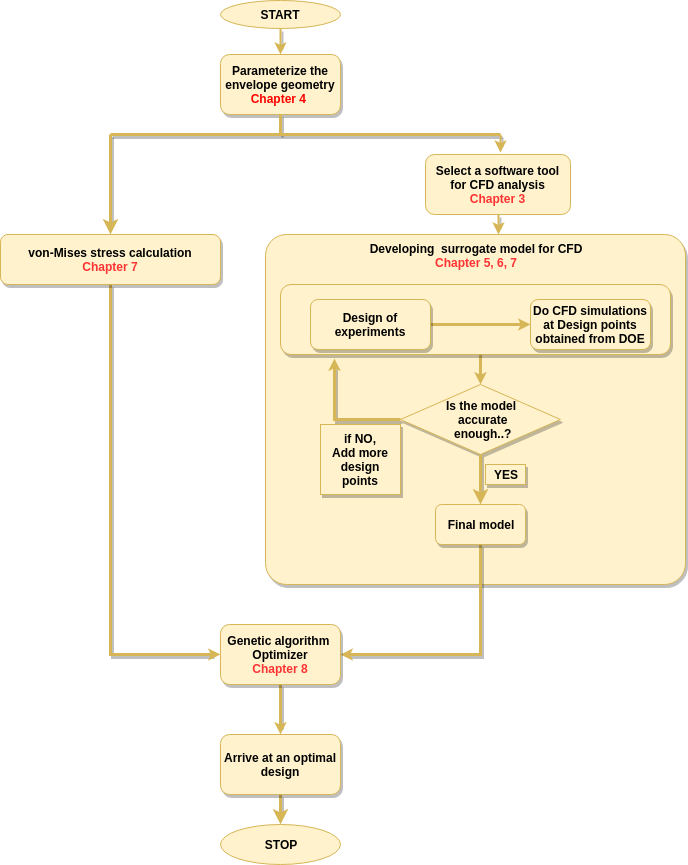
\includegraphics[width=\textwidth]{layout/report_layout.png} 
	\caption{Framework of multi-disciplinary shape optimization}
	\label{Report layout} %      only if needed 	
\end{figure}
%%
The next Chapter gives brief literature survey that has been carried out to understand the previous research carried out in the field of High Altitude Airships (HAA's) and shape optimization.


%%% Local Variables: 
%%% mode: latex
%%% TeX-master: "../mainrep"
%%% End: 

%%


%%% Local Variables: 
%%% mode: latex
%%% TeX-master: "../mainrep"
%%% End: 
